\documentclass[11pt]{article}\usepackage[]{graphicx}\usepackage[]{color}
%% maxwidth is the original width if it is less than linewidth
%% otherwise use linewidth (to make sure the graphics do not exceed the margin)
\makeatletter
\def\maxwidth{ %
  \ifdim\Gin@nat@width>\linewidth
    \linewidth
  \else
    \Gin@nat@width
  \fi
}
\makeatother

\definecolor{fgcolor}{rgb}{0.345, 0.345, 0.345}
\newcommand{\hlnum}[1]{\textcolor[rgb]{0.686,0.059,0.569}{#1}}%
\newcommand{\hlstr}[1]{\textcolor[rgb]{0.192,0.494,0.8}{#1}}%
\newcommand{\hlcom}[1]{\textcolor[rgb]{0.678,0.584,0.686}{\textit{#1}}}%
\newcommand{\hlopt}[1]{\textcolor[rgb]{0,0,0}{#1}}%
\newcommand{\hlstd}[1]{\textcolor[rgb]{0.345,0.345,0.345}{#1}}%
\newcommand{\hlkwa}[1]{\textcolor[rgb]{0.161,0.373,0.58}{\textbf{#1}}}%
\newcommand{\hlkwb}[1]{\textcolor[rgb]{0.69,0.353,0.396}{#1}}%
\newcommand{\hlkwc}[1]{\textcolor[rgb]{0.333,0.667,0.333}{#1}}%
\newcommand{\hlkwd}[1]{\textcolor[rgb]{0.737,0.353,0.396}{\textbf{#1}}}%
\let\hlipl\hlkwb

\usepackage{framed}
\makeatletter
\newenvironment{kframe}{%
 \def\at@end@of@kframe{}%
 \ifinner\ifhmode%
  \def\at@end@of@kframe{\end{minipage}}%
  \begin{minipage}{\columnwidth}%
 \fi\fi%
 \def\FrameCommand##1{\hskip\@totalleftmargin \hskip-\fboxsep
 \colorbox{shadecolor}{##1}\hskip-\fboxsep
     % There is no \\@totalrightmargin, so:
     \hskip-\linewidth \hskip-\@totalleftmargin \hskip\columnwidth}%
 \MakeFramed {\advance\hsize-\width
   \@totalleftmargin\z@ \linewidth\hsize
   \@setminipage}}%
 {\par\unskip\endMakeFramed%
 \at@end@of@kframe}
\makeatother

\definecolor{shadecolor}{rgb}{.97, .97, .97}
\definecolor{messagecolor}{rgb}{0, 0, 0}
\definecolor{warningcolor}{rgb}{1, 0, 1}
\definecolor{errorcolor}{rgb}{1, 0, 0}
\newenvironment{knitrout}{}{} % an empty environment to be redefined in TeX

\usepackage{alltt}
\usepackage{amsmath}
\usepackage{amssymb}
\usepackage{geometry}
\usepackage{graphicx}
\usepackage{bm}
\usepackage{url}
\usepackage{enumerate}
\usepackage{hyperref}
\IfFileExists{upquote.sty}{\usepackage{upquote}}{}
\begin{document}

\setlength\parindent{0pt}

\Large \textbf{Lab 1: Simple Linear Regression in R}\\
\large \textbf{STAT 632, Spring 2020}
\normalsize

\section{Data Set}
For this lab we consider a data set called \texttt{fandango} from the R package \texttt{fivethirtyeight}.  The data set contains a sample of movie ratings from Fandango, Rotten Tomatoes, Metacritic, and IMDb.  The data was used for the FiveThirtyEight article \href{https://fivethirtyeight.com/features/fandango-movies-ratings/}{Be Suspicious Of Online Movie Ratings, Especially Fandango’s}.  The article argues that the movie ratings on Fandango tend to be higher than other websites.\\

First, to install the package run the command:
\begin{knitrout}
\definecolor{shadecolor}{rgb}{0.969, 0.969, 0.969}\color{fgcolor}\begin{kframe}
\begin{alltt}
\hlkwd{install.packages}\hlstd{(}\hlstr{"fivethirtyeight"}\hlstd{)}
\end{alltt}
\end{kframe}
\end{knitrout}
You only need to install a package on your computer once.  Next, to load the contents of the package into RStudio run the command:
\begin{knitrout}
\definecolor{shadecolor}{rgb}{0.969, 0.969, 0.969}\color{fgcolor}\begin{kframe}
\begin{alltt}
\hlkwd{library}\hlstd{(fivethirtyeight)}
\end{alltt}
\end{kframe}
\end{knitrout}
Note that you need to run the \texttt{library()} command each time you open RStudio and want to use a particular package.  The \texttt{fandango} data set should now be available in RStudio.  Try previewing the first several rows of this data frame:
\begin{knitrout}
\definecolor{shadecolor}{rgb}{0.969, 0.969, 0.969}\color{fgcolor}\begin{kframe}
\begin{alltt}
\hlkwd{head}\hlstd{(fandango)}
\end{alltt}
\end{kframe}
\end{knitrout}
You can also read about this data set in the help menu by entering the command: 
\begin{knitrout}
\definecolor{shadecolor}{rgb}{0.969, 0.969, 0.969}\color{fgcolor}\begin{kframe}
\begin{alltt}
\hlkwd{help}\hlstd{(fandango)}
\end{alltt}
\end{kframe}
\end{knitrout}

In this lab, we will use simple linear regression to model the relationship between the variables \texttt{fandango\_ratingvalue} and \texttt{imdb\_norm}.  Note that the IMDb ratings have been normalized between 0 and 5 so that they can be compared directly with Fandango ratings.\\

A good place to start, before actually fitting a model, is to look at some descriptive statistics of the variables.
\begin{knitrout}
\definecolor{shadecolor}{rgb}{0.969, 0.969, 0.969}\color{fgcolor}\begin{kframe}
\begin{alltt}
\hlkwd{summary}\hlstd{(fandango}\hlopt{$}\hlstd{fandango_ratingvalue)}
\end{alltt}
\begin{verbatim}
##    Min. 1st Qu.  Median    Mean 3rd Qu.    Max. 
##   2.700   3.500   3.900   3.845   4.200   4.800
\end{verbatim}
\begin{alltt}
\hlkwd{summary}\hlstd{(fandango}\hlopt{$}\hlstd{imdb_norm)}
\end{alltt}
\begin{verbatim}
##    Min. 1st Qu.  Median    Mean 3rd Qu.    Max. 
##   2.000   3.150   3.450   3.368   3.700   4.300
\end{verbatim}
\end{kframe}
\end{knitrout}

\section{Simple Linear Regression Model}
Use the \texttt{lm()} function to fit a simple linear regression model.  
\begin{knitrout}
\definecolor{shadecolor}{rgb}{0.969, 0.969, 0.969}\color{fgcolor}\begin{kframe}
\begin{alltt}
\hlstd{lm1} \hlkwb{<-} \hlkwd{lm}\hlstd{(fandango_ratingvalue} \hlopt{~} \hlstd{imdb_norm,} \hlkwc{data} \hlstd{= fandango)}
\end{alltt}
\end{kframe}
\end{knitrout}
The function uses the formula notation $y \sim x$, where $y$ is the response variable\\ (\texttt{fandango\_ratingvalue}) and $x$ is the explanatory variable (\texttt{imdb\_norm}).\\

Use the \texttt{summary()} function to print out important information about the linear regression model we just fit.
\begin{knitrout}
\definecolor{shadecolor}{rgb}{0.969, 0.969, 0.969}\color{fgcolor}\begin{kframe}
\begin{alltt}
\hlkwd{summary}\hlstd{(lm1)}
\end{alltt}
\begin{verbatim}
## 
## Call:
## lm(formula = fandango_ratingvalue ~ imdb_norm, data = fandango)
## 
## Residuals:
##      Min       1Q   Median       3Q      Max 
## -0.99653 -0.26402 -0.01228  0.30208  1.07577 
## 
## Coefficients:
##             Estimate Std. Error t value Pr(>|t|)    
## (Intercept)  1.72393    0.23784   7.248 2.37e-11 ***
## imdb_norm    0.62974    0.06991   9.008 1.16e-15 ***
## ---
## Signif. codes:  0 '***' 0.001 '**' 0.01 '*' 0.05 '.' 0.1 ' ' 1
## 
## Residual standard error: 0.4035 on 144 degrees of freedom
## Multiple R-squared:  0.3604,	Adjusted R-squared:  0.356 
## F-statistic: 81.15 on 1 and 144 DF,  p-value: 1.155e-15
\end{verbatim}
\end{kframe}
\end{knitrout}
\clearpage

The least squares estimates of the slope and intercept are given in the \texttt{Coefficients} table of the summary output.  The equation of the least squares regression line can therefore be written as
$$\hat{y} =  1.7239 + 0.62974x$$
The summary output gives an $R^2 = 0.3604$.  This means that 36.04\% of the variation in fandango ratings can be explained by the IMDb ratings.\\

Next, we can make a scatterplot of our data and superimpose the least squares regression line.  The 1-1 line (i.e., the $y=x$ line) is also plotted for comparison.
\begin{knitrout}
\definecolor{shadecolor}{rgb}{0.969, 0.969, 0.969}\color{fgcolor}\begin{kframe}
\begin{alltt}
\hlkwd{plot}\hlstd{(fandango_ratingvalue} \hlopt{~} \hlstd{imdb_norm,} \hlkwc{data} \hlstd{= fandango,}
     \hlkwc{ylab} \hlstd{=} \hlstr{"Fandango Rating"}\hlstd{,} \hlkwc{xlab}\hlstd{=}\hlstr{"IMDb Rating"}\hlstd{,}
     \hlkwc{xlim}\hlstd{=}\hlkwd{c}\hlstd{(}\hlnum{2}\hlstd{,}\hlnum{4.8}\hlstd{),} \hlkwc{ylim} \hlstd{=} \hlkwd{c}\hlstd{(}\hlnum{2}\hlstd{,}\hlnum{4.8}\hlstd{))}
\hlkwd{abline}\hlstd{(lm1)} \hlcom{# add regression line}
\hlkwd{abline}\hlstd{(}\hlnum{0}\hlstd{,} \hlnum{1}\hlstd{,} \hlkwc{lty}\hlstd{=}\hlnum{2}\hlstd{)} \hlcom{# add 1-1 line}
\end{alltt}
\end{kframe}
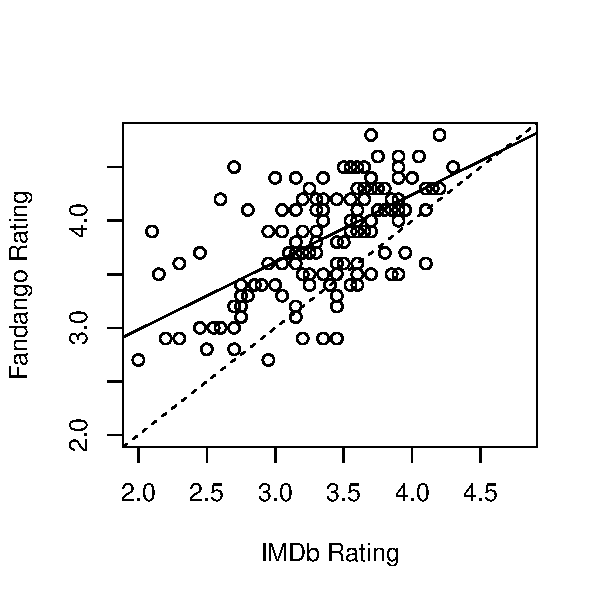
\includegraphics[width=\maxwidth]{figure/unnamed-chunk-8-1} 

\end{knitrout}

The scatter plot shows that Fandango movie ratings tend to be higher than IMDb; this agrees with the conclusions from the FiveThirtyEight article.  Specifically, the regression line is above the 1-1 line, indicating that Fandango ratings are higher than IMDb, on average, especially for movies that are rated poorly on IMDb.

\section{Attributes from \texttt{lm} Objects}
The linear model object we created has various attributes that we can extract by name.     
\begin{knitrout}
\definecolor{shadecolor}{rgb}{0.969, 0.969, 0.969}\color{fgcolor}\begin{kframe}
\begin{alltt}
\hlkwd{attributes}\hlstd{(lm1)}
\end{alltt}
\begin{verbatim}
## $names
##  [1] "coefficients"  "residuals"     "effects"       "rank"         
##  [5] "fitted.values" "assign"        "qr"            "df.residual"  
##  [9] "xlevels"       "call"          "terms"         "model"        
## 
## $class
## [1] "lm"
\end{verbatim}
\begin{alltt}
\hlcom{# extract coefficients (parameter estimates)}
\hlkwd{coef}\hlstd{(lm1)}
\end{alltt}
\begin{verbatim}
## (Intercept)   imdb_norm 
##    1.723934    0.629739
\end{verbatim}
\begin{alltt}
\hlcom{# extract residuals}
\hlkwd{head}\hlstd{(}\hlkwd{resid}\hlstd{(lm1))}
\end{alltt}
\begin{verbatim}
##            1            2            3            4            5 
##  0.320083951  0.540492586  0.320083951  1.075770701 -0.329768456 
##            6 
##  0.009005639
\end{verbatim}
\begin{alltt}
\hlcom{# extract fitted (predicted) values}
\hlkwd{head}\hlstd{(}\hlkwd{predict}\hlstd{(lm1))}
\end{alltt}
\begin{verbatim}
##        1        2        3        4        5        6 
## 4.179916 3.959507 4.179916 3.424229 3.329768 3.990994
\end{verbatim}
\begin{alltt}
\hlcom{# 95% confidence intervals for intercept and slope}
\hlkwd{confint}\hlstd{(lm1)}
\end{alltt}
\begin{verbatim}
##                 2.5 %    97.5 %
## (Intercept) 1.2538337 2.1940345
## imdb_norm   0.4915635 0.7679144
\end{verbatim}
\end{kframe}
\end{knitrout}
\clearpage

\subsection{Model Diagnostics}
A useful diagnostic is a plot of the residuals versus the fitted values.  Use the \texttt{predict()} function to extract the fitted values ($\hat{y}_i$); and use the \texttt{resid()} function to extract the residuals ($\hat{e}_i = y_i - \hat{y_i}$).
\begin{knitrout}
\definecolor{shadecolor}{rgb}{0.969, 0.969, 0.969}\color{fgcolor}\begin{kframe}
\begin{alltt}
\hlkwd{par}\hlstd{(}\hlkwc{mar}\hlstd{=}\hlkwd{c}\hlstd{(}\hlnum{4}\hlstd{,}\hlnum{4}\hlstd{,}\hlnum{1}\hlstd{,}\hlnum{1}\hlstd{),} \hlkwc{mfrow}\hlstd{=}\hlkwd{c}\hlstd{(}\hlnum{1}\hlstd{,}\hlnum{2}\hlstd{))} \hlcom{# adjust margins, and split graphics pane}
\hlcom{# residual plot}
\hlkwd{plot}\hlstd{(}\hlkwd{predict}\hlstd{(lm1),} \hlkwd{resid}\hlstd{(lm1),} \hlkwc{xlab}\hlstd{=}\hlstr{"Fitted values"}\hlstd{,} \hlkwc{ylab}\hlstd{=}\hlstr{"Residuals"}\hlstd{)}
\hlkwd{abline}\hlstd{(}\hlkwc{h}\hlstd{=}\hlnum{0}\hlstd{)}
\hlcom{# histogram of residuals}
\hlkwd{hist}\hlstd{(}\hlkwd{resid}\hlstd{(lm1),} \hlkwc{main}\hlstd{=}\hlstr{""}\hlstd{,} \hlkwc{xlab}\hlstd{=}\hlstr{"Residuals"}\hlstd{)}
\end{alltt}
\end{kframe}
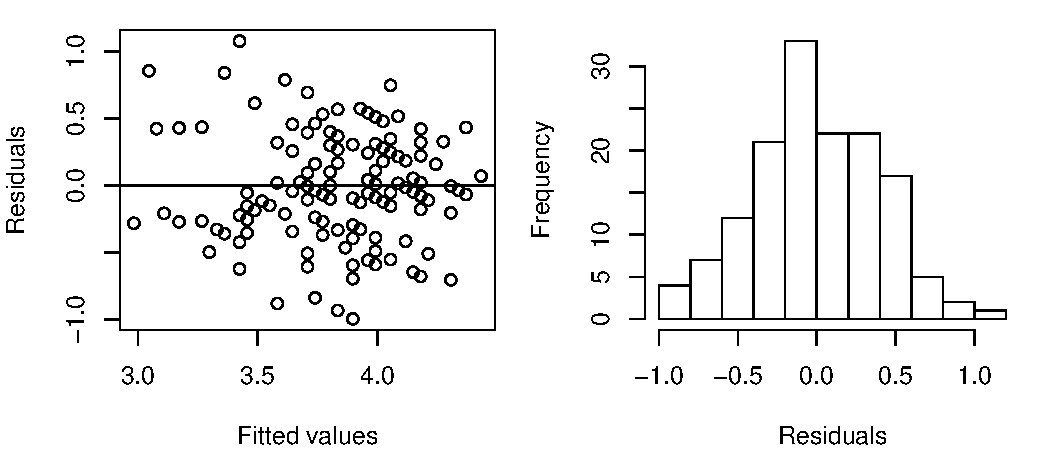
\includegraphics[width=\maxwidth]{figure/unnamed-chunk-10-1} 

\end{knitrout}

The points in the residual plot appear randomly scattered around 0.  There are no outliers, or indications of nonlinearity or nonconstant variance.  The histogram of the residuals also appears normally distributed.  Therefore, the conditions for simple linear regression appear to be well satisfied.\\
\clearpage

\section{Making Predictions}
We can use the \texttt{predict()} function to make predictions at new values of the explanatory variable.  Recall, that the least squares regression line for predicting a movie's Fandango rating from the IMDb normalized rating is
$$\hat{y} =  1.7239 + 0.62974x$$
For example, the predicted Fandango rating for a movie with an IMDb normalized rating of $x=4$ is given by
$$\hat{y} =  1.7239 + 0.62974(4) = 4.24286$$
We can do this calculation in R with the following command:
\begin{knitrout}
\definecolor{shadecolor}{rgb}{0.969, 0.969, 0.969}\color{fgcolor}\begin{kframe}
\begin{alltt}
\hlstd{new_x} \hlkwb{<-} \hlkwd{data.frame}\hlstd{(}\hlkwc{imdb_norm} \hlstd{=} \hlnum{4}\hlstd{)}
\hlkwd{predict}\hlstd{(lm1,} \hlkwc{newdata} \hlstd{= new_x)}
\end{alltt}
\begin{verbatim}
##       1 
## 4.24289
\end{verbatim}
\end{kframe}
\end{knitrout}
which gives the same result as the manual calculation.\\

We can also use this approach to make several predictions at once.  For example, the following command gives the predicted Fandango ratings for movies with IMDb normalized ratings of $x=2.5, 3.5, 4.5$.
\begin{knitrout}
\definecolor{shadecolor}{rgb}{0.969, 0.969, 0.969}\color{fgcolor}\begin{kframe}
\begin{alltt}
\hlstd{new_x} \hlkwb{<-} \hlkwd{data.frame}\hlstd{(}\hlkwc{imdb_norm} \hlstd{=} \hlkwd{c}\hlstd{(}\hlnum{2.5}\hlstd{,}\hlnum{3.5}\hlstd{,}\hlnum{4.5}\hlstd{))}
\hlkwd{predict}\hlstd{(lm1,} \hlkwc{newdata} \hlstd{= new_x)}
\end{alltt}
\begin{verbatim}
##        1        2        3 
## 3.298282 3.928020 4.557759
\end{verbatim}
\end{kframe}
\end{knitrout}

The \texttt{predict()} function can also be used to compute a 95\% prediction interval (more on this next class).

\begin{knitrout}
\definecolor{shadecolor}{rgb}{0.969, 0.969, 0.969}\color{fgcolor}\begin{kframe}
\begin{alltt}
\hlstd{new_x} \hlkwb{<-} \hlkwd{data.frame}\hlstd{(}\hlkwc{imdb_norm} \hlstd{=} \hlnum{4}\hlstd{)}
\hlkwd{predict}\hlstd{(lm1,} \hlkwc{newdata} \hlstd{= new_x,} \hlkwc{interval} \hlstd{=} \hlstr{"prediction"}\hlstd{)}
\end{alltt}
\begin{verbatim}
##       fit      lwr      upr
## 1 4.24289 3.437823 5.047957
\end{verbatim}
\end{kframe}
\end{knitrout}
\clearpage
Here's how to make the scatterplot with the least squares line using \texttt{ggplot2}.

\begin{knitrout}
\definecolor{shadecolor}{rgb}{0.969, 0.969, 0.969}\color{fgcolor}\begin{kframe}
\begin{alltt}
\hlkwd{library}\hlstd{(ggplot2)}
\hlkwd{ggplot}\hlstd{(fandango,} \hlkwd{aes}\hlstd{(imdb_norm, fandango_ratingvalue))} \hlopt{+}
  \hlkwd{geom_point}\hlstd{()} \hlopt{+} \hlkwd{geom_smooth}\hlstd{(}\hlkwc{method} \hlstd{=} \hlstr{"lm"}\hlstd{,} \hlkwc{se} \hlstd{=} \hlnum{FALSE}\hlstd{)} \hlopt{+}
  \hlkwd{xlab}\hlstd{(}\hlstr{"IMDb Rating"}\hlstd{)} \hlopt{+} \hlkwd{ylab}\hlstd{(}\hlstr{"Fandango Rating"}\hlstd{)}
\end{alltt}
\end{kframe}
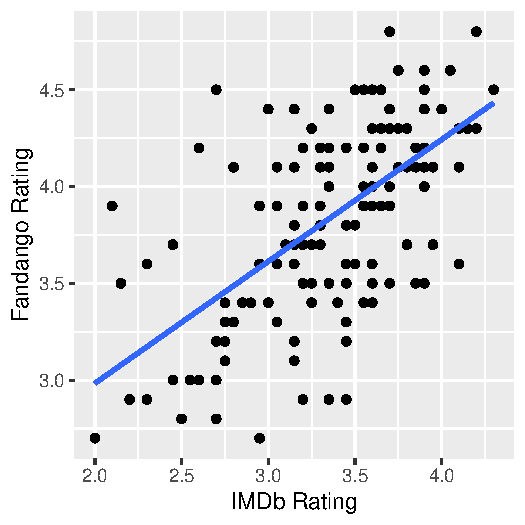
\includegraphics[width=\maxwidth]{figure/unnamed-chunk-14-1} 

\end{knitrout}









\end{document}
